\documentclass[aspectratio=43]{beamer}
\usetheme{Berlin}

\title{Sample Title}
\subtitle{Sample Subtitle}
\usepackage[czech]{babel}
\usecolortheme{dolphin}
\usepackage{graphicx}
\usepackage{dirtree}
\usepackage{listings}
\usepackage[utf8]{inputenc}
\usepackage{caption}		% popisky

\captionsetup{labelformat=empty}

\defbeamertemplate*{title page}{customized}[1][]
{
	\usebeamerfont{title}\inserttitle\par
	\usebeamerfont{subtitle}\usebeamercolor[fg]{subtitle}\insertsubtitle\par
	\bigskip
	\usebeamerfont{author}\insertauthor\par
	\usebeamerfont{institute}\insertinstitute\par
	\usebeamerfont{date}\insertdate\par
	\usebeamercolor[fg]{titlegraphic}\inserttitlegraphic
}

\hypersetup{unicode}
\hypersetup{breaklinks=true}

\usepackage{color}
\definecolor{pblue}{rgb}{0.13,0.13,1}
\definecolor{pgreen}{rgb}{0,0.5,0}
\definecolor{pred}{rgb}{0.9,0,0}
\definecolor{pgrey}{rgb}{0.46,0.45,0.48}




\title{AvAvA -- Kontejnerizační systém pro Linux}
\subtitle{Ročníková práce}
\author{Havránek Kryštof, Josef Litoš, Vladimír Vávra 3.E}
\date{29. května 2021}
\institute{Gymnázium, Arabská 14, Praha 6}
\setbeamertemplate{sidebar right}{}
\setbeamertemplate{footline}{%
\hfill\textbf{\insertframenumber{}/\inserttotalframenumber}}


\begin{document}
\begin{frame}[plain]
	\maketitle
\end{frame}
\frame{
	\frametitle{Úvod}
	\section{Úvod}
	\begin{itemize}
		\item AvAvA -- Kontejnerizační systém pro Linux
		\item Zdrojový kód na GitHubu pod licencí GPLv3
		\item Rozdělení Práce
			\begin{itemize}
				\item Kryštof -- Databáze a routy
				\item Josef -- propojení s LXD
				\item Vladimír -- Frontend
				\item všichni -- API
			\end{itemize}
		\item Spolupráce: Discord, Github
	\end{itemize}

}
\frame{
	\frametitle{Hlavní funkce}
	\section{Funkce}
	\begin{itemize}
		\item Možnost vytvořit a smazat kontejnery a projekty. % \item Kontejnery vždy musí mít specifikované limity, projekty mohou.
		\item Změna limitů a dalších nastavitelných možností.
		\item Přehledné zobrazení informací a aktuálního stavu u kontejnerů, projektů i uživatele
		\item Připojení určitých portů kontejneru k internetu pomocí subdomény
	\end{itemize}
}
\frame{
	\frametitle{Vedlejší funkce}
	\begin{itemize}
		\item Vytvoření a stažení zálohy kontejneru
		\item Integrovaný terminál pro správu kontejneru přímo z aplikace.
		\item Logování stavu každých pro vykreslování dlouhodobého stavu kontejneru
	\end{itemize}
}

\frame{
	\frametitle{Architektura}
	\section{Architektura}
	\centering
	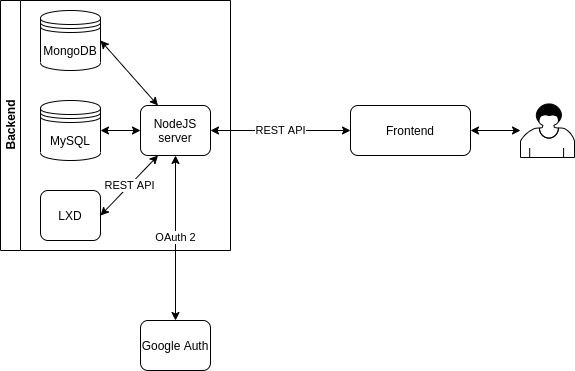
\includegraphics[height=6cm]{../img/architecture.png} % websocket
}
\frame{
	\frametitle{Autentifikace}
	\centering
	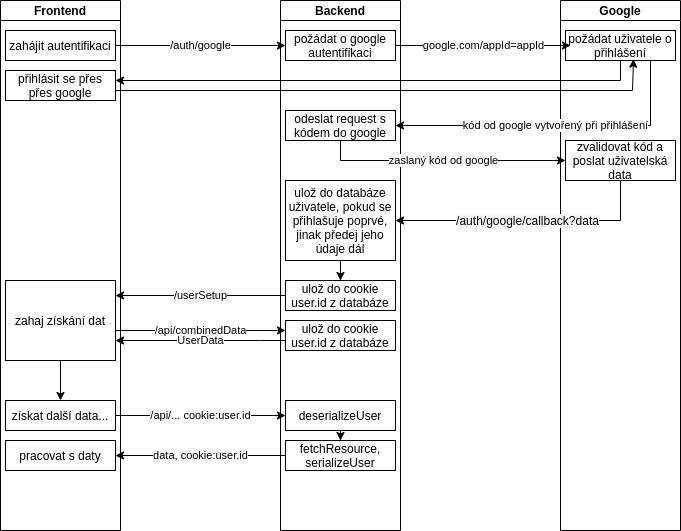
\includegraphics[height=6cm]{../img/authentication.png}% vládis, co se dělá na beckendu
}


\frame{
	\frametitle{Frontend}
	\section{Frontend}
	\begin{itemize}
		\item ReactJS, SASS, JavaScript, Redux
		\item použité knihovny: react-bootstrap, material-ui, react-router, superagent, ...
		\item základ -- template
	\end{itemize}

}
\frame{
	\frametitle{Backend}
	\section{Backend}
	\begin{itemize}
		\item NodeJS, JavaScript, express
		\item mongoDB, mySQL
		\item LXD
		\item HAProxy
	\end{itemize}
}

\frame{
	\frametitle{Backend -- LXD}
	\begin{itemize}
		\item podpora přímo v kernelu linuxu
		\item nejefektivnější způsob sdílení zdrojů
		\item limity % přímo podporované lxd
		\item lxdRoute.js $\Rightarrow$ REST API
	\end{itemize}
}

\frame{
	\frametitle{Backend -- Databáze -- SQL}
	\begin{itemize}
		\item mariaDB
		\item veškerá data o uživatelích, projektech a kontejnerech
		\item logy
		\item v programu s ní zachází 4 třídy
	\end{itemize}
}

\frame{
	\frametitle{Backend -- Databáze -- SQL}
	\centering
	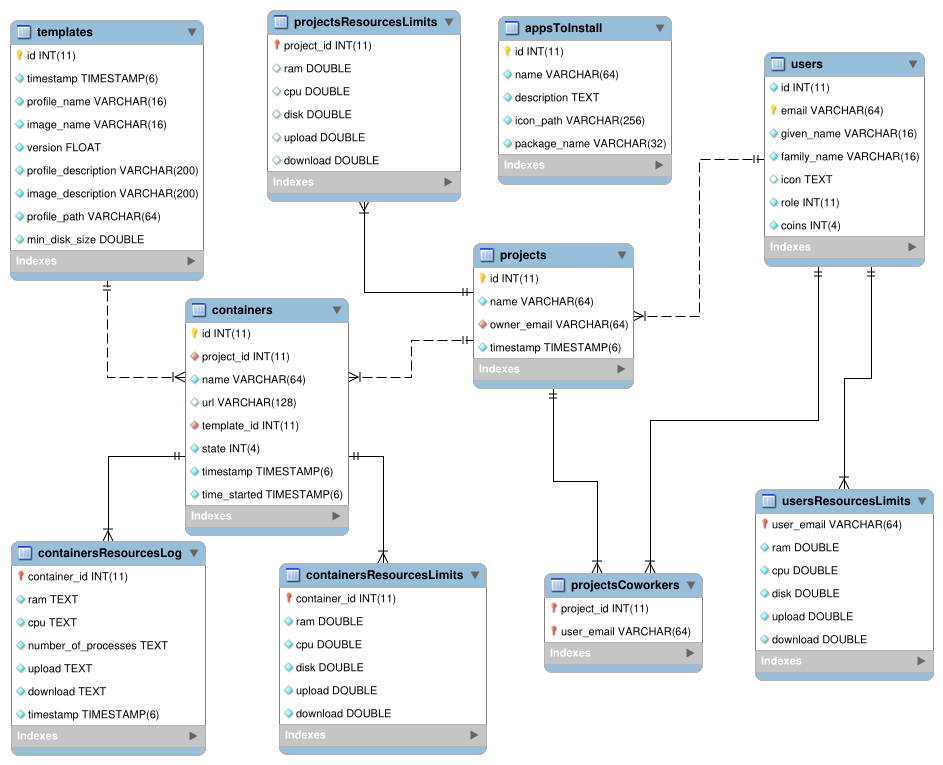
\includegraphics[height=7cm]{../img/lolwut.png}% vládis, co se dělá na beckendu
}

\frame{
	\frametitle{Backend -- Databáze -- mongoDB}
	\begin{itemize}
		\item problémy s získáním stavu vypnutého kontejneru
		\item zapisuje se vždy při změně stavu, nebo přečtení stavu
		\item organizace:
			\begin{itemize}
				\item kolekce -- projekty
				\item tabulky v nich -- stav kontejneru
			\end{itemize}
	\end{itemize}
}

\frame{
	\frametitle{Backend -- HAProxy}
	\begin{itemize}
		\item problém zpřístupnění kontejnerů na internetu % lze mezi nimi však komunikovat, jelikož s našem nastavení jsou veškeré kontejnery na stejné síti a lxd samo přiřazuje jim na ní doménu
		\item HAProxy -- sólo kontejner % TCP proxy, host přeposílá 80, 443, 2000, 2222, 3000, 5000
		\item doména ve tvaru \textit{\{jméno kontejneru\}.\{jméno projektu\}.\{část emailu uživatel, před @\}.\{doména serveru\}}
		\item potíže se směrováním $\Rightarrow$  u ssh nutný proxy command % SNI není součástí packetu u řady protokolů, proxy, neví kam posílat
		\item generace konfigurace v containerSQL.js, automatické nahrání do kontejneru
	\end{itemize}
}
\frame{
	\frametitle{Závěr}
	\section{Závěr} % po ukázce zda byla práce úspěšná
	\begin{itemize}
		\item Většina funkcí aktuálního api byla implementována
		\item S úpravami je možné jeho nasazení
	\end{itemize}
}
\frame{
	\frametitle{Budoucnost Projektu}
	\begin{itemize}
		\item dokončení všech rozpracovaných funkcí - Snapshoty, Vykreslování historie grafů u kontejnerů a projektů
		\item administrátorský a superadministrátorský účet - nové funkce: správa imagů, profilů, uživatelů a jejich kontejnerů
		\item real-time systém -- websocket
		\item kooperace uživatelů - možnost vytvoření sdílených projektů
		\item možnost navyšovat zdroje uživatele a integrace základní ekonomiky
		\item zjištění limitů, při kterých kontejnery dobře fungují
		\item deploynutí na školní server
		\item SOČ
	\end{itemize}
}

\end{document}
